\chapter{Implementation Tree Edit Distance}
In this chapter we present the implementation of Shasha and Zhangs algorithm by Henderson~\cite{Hen}. We discuss meaningful choices of cost functions and compare them with each other. Last but not least we compare the tree edit distance's advantages and disadvantages with respect to the Generalized Robinson Foulds distance. 

\section{Shasha and Zhang's algorithm by Henderson}
Suppose we want to compute the tree edit distance for two trees $A$ and $B$. Henderson's implementation can be split into two separated important steps:
\begin{enumerate}
\item Finding out the post-order traversal index and the keyroots for the two trees under consideration.
\item Computing the tree edit distances for all relevant subproblems, i.e. combinations of subtrees induced by keyroots of $A$ and $B$ respectively.
\end{enumerate}

\underline{Ad Step $1$}:\\
In Listing~\ref{lst:AnnTree} we present the initialization of the class AnnotatedTree. It can be split up into two parts: Step $1$a) and Step $1$b). We will give a short summary of what happens in these two substeps later on.
\lstinputlisting[language=Python, caption=Initialization of an AnnotatedTree, label=lst:AnnTree]{figures/annotated_tree.py}
\underline{Ad Step $1$a)}:\\
This substep initializes a stack $pstack$ that is needed for the Step $1$b). But first we take a close look at the variable called $stack$. A stack is a specific data structure. It is a collection of objects that supports fast last-in, first-out semantics. Throughout the process of the loop, the stack always consists of a pair of data, namely a node and a list of all its ancestors. Therefore we initialize the stack with the pair of the annotated tree's root and an empty collection, since the root doesn't have an ancestor. \\
While the stack still contains some pair of data we perform a function on it called \textit{pop}. This function returns the last element of the stack and removes it from the stack. We associate every node with a unique id $nid$. If the inspected node has some children we enlarge the stack with pairs of each children and the updated list of ancestors. The essential detail is that we \textit{append} this pair to the stack, which means that we put it on the end of the stack. The reason why this is so important will be explained later. After appending all children to the stack, the node will be appended to another stack called $pstack$ which will be used in Step $1$b), together with its node id $nid$ and the list of ancestors.
Let's go through the process for the first pair of data, namely the root and the empty set of ancestors. We assign the $nid$ $0$ to the root and go through its children. Here we first append the root's left child, afterwards its right child. Thus the right child is further in the back of the stack than the left child. Since we only $pop$ the stack, the right child will be out of the stack earlier than the left child. Furthermore, during the next loop we append the stack with other nodes again, pushing the left child of the root further down the stack. Thus we end up with the new stack $pstack$ that has the correct left to right post traversal ordering. The further back a node is in the stack $pstack$, the smaller is its post traversal ordering index.
\\
\underline{Ad Step $1$b)}:\\
In this step we determine the keyroots of the investigated tree. The key idea is, that a node is a keyroot if and only if it is the node with the highest post-order traversal index among all nodes with the same left most descendant. The right sibling of a node $n$ has a different left most descendant than the node $n$ itself. But any node with a higher index can not have the same left most descandant as this right sibling because of the way we indexed the nodes. Thus if we determine the node with the highest index among all nodes that share the same leftmost descendant, then we know that it has to be a keyroot. For this we need two temporary dictionaries $lmds$, the list of the left most descendant for every node, and $keyroots$, a dictionary that saves the highest index of all nodes that share a leftmost descendant.\\
As previously discussed we go through $pstack$, a stack of nodes in the correct order. The counter $i$ saves the actual post order index, it increments after every loop. 
During every loop we pop the stack and get a node $n$, its node id $nid$ and its ancestors. Then we check whether the node is a leaf or not. If it indeed is, then we set the left most descendant of every ancestor to this node, as long as it does not already have a left most descendant. If it is an interior node, then we just get the left most descendant by checking the dictionary $lmds$. The most important step happens near the end of the loop: setting $keyroots[lmd] = i$. In this way we find the highest index $i$ of all nodes, that share the same leftmost descendant. Therefore, after having finished the routine, we get the keyroots by checking the values of the temporary dictionary $keyroots$.

This was a detailed description of the way an object of type AnnotatedTree gets initialized. It makes use of efficiently appending and popping a stack to receive the correct indexing and the all the necessary information to get the list of keyroots.

\underline{Ad Step $2$}:\\
After the initialization of the AnnotatedTree, the actual computation of the tree edit distance is done by first considering all relevant subproblems. A distance matrix is created that stores the pairwise distance between all relevant subproblems of the two investigated trees. This matrix gets built incrementally by applying the recursion stated in Lemma~\ref{lem:saz}. The technical details can be seen in the actual implementation~\cite{Hen}.

\section{Distance measures}
The most simple distance measure for the tree edit distance just counts the number of operations needed to transform one tree into the other. This implies that any insertion, any deletion and any renaming costs the same value of $1$. We call this distance measure the \textit{standard tree edit distance} (STED)\\
The big difference between the tree edit distance and the generalized Robinson Foulds is that the latter does not take the interior nodes of the trees into account. Yet every insertion and deletion of an interior node increases the tree edit distance. Therefore the first adaption on the operation costs we did was to make the insertion and deletion of interior nodes free of charge. We will later see how this influences the overall comparison between these two distances. This distance measure will later be referred to as \textit{cheap tree edit distance} (CTED)\\
Another distinction is that the Robinson Foulds distance doesn't make a difference between left and right. Therefore there was an attempt to improve the distance measure by adapting the direction. The idea is to change one of the trees by swapping the order among some sibling pairings. Considering all combinations of sibling pairings leeds to $O(2^n)$ possibilities of swapping siblings, which is obviously not a good solution. To explain our approach we consider the two roots $r_1$ and $r_2$ of the inspected trees.
Let's denote the left subtree of the root $r_i$ as $L_i$ and the right one as $R_i$ for $i \in \{1,2\}$. If $|L_1| > |R_1|$, meaning that $L_1$ has more leaves than $R_1$, but the opposite holds true for the other tree, i.e. $|L_2| < |R_2|$, then we swap the children of $r_1$. The goal is to make the two trees as equally distributed as possible without changing the set of clusters for these randomly created trees. Thus the Robinson Foulds distance stays the same, but the tree edit distance may change. After having investigated the root we perform the same comparison between $l_1$ and $l_2$, $r_1$ and $r_2$ respectively. If we adapt one of the trees to make them as equally distributed as possible before calculating, we add the adjective \textit{adapted} to the distance. So later on we will refer to it as the \textit{adapted standard tree edit distance} (aSTED) and the \textit{adapted cheap tree edit distance} (aCTED).\\
Furthermore we wanted to investigate a compromise bewteen the CTED and the STED by varying the costs of insertion and deletion of inner nodes. We introduced a variable $0 < \delta < 1$ for the costs of insertion and deletion. Assuming $\delta = \frac{1}{2}$,  we call this distance measure $\frac{1}{2}$-\textit{delta tree edit distance} ($\frac{1}{2}$-DTED).

\section{Results}
For smaller trees we were able to compare the results with the ones from the generalized Robinson Foulds distance. But for trees with more than $32$ leaves it was not possible to solve the linear program, as this would have taken too much time. However we were able to compute the tree edit distance for trees with up to $512$ leaves. 

Obviously, we came to the conclusion that the STED lead to bigger distance values than the CTED. This is trivial as every operation is as least as expensive for the STED in comparison to the CTED. Furthermore, to get a better feeling, we put the distances in relation to the number of leaves. From now on we denote the number of leaves on each tree as the variable $n$. We discovered two trends as $n$ is increasing:
\begin{itemize}
\item The average of the relation of the CTED to $n$ is diverging to $1$.
\item The average of the relation of the STED to $n$ among all examples is strongly increasing.
\end{itemize}
The explanation for the first trend is rather intuitive. Figure~\ref{fig:CTED} indicates that any tree has distance $\leq n$ to any other tree on the same number of leaves $n$.
\begin{figure}[!h]
    \centering
        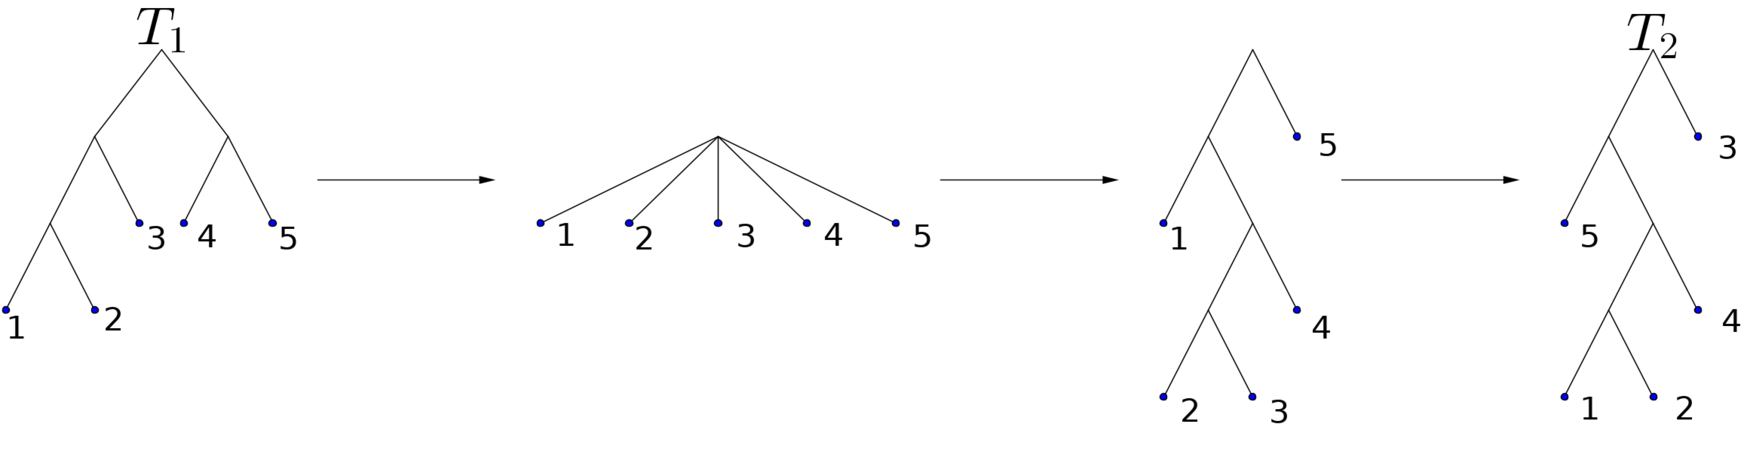
\includegraphics[width=0.90\textwidth]{figures/CTED.png}
        \caption{A step guide for limiting the CTED. First we delete all inner nodes until all leaves are directly connected to the root. Afterwards we insert all inner nodes until the structure is the same as the one of tree $T_2$. Now we only have to rename all leaves accordingly. Since the deletion and insertion of inner nodes is for free we end up with a CTED $\leq n$.}
        \label{fig:CTED}
\end{figure}
Since the CTED converges to $n$ it seems as if this distance is not a good measure of similarities between structure of the two trees at all, but only whether the order of the leaves' labels is similar.\\
Thus we investigated the DTED, mainly with $\delta = \frac{1}{2}$, and observed some interesting behaviors. For example, The distribution of the relation of the $\frac{1}{2}$-DTED to $n$ becomes more and more constant as $n$ is increasing. 


\section{Comparing Results}
